\section{Muhammad Reza Syachrani (1174084)}
\subsection{Menulis Shapefile dengan PySHP}
\begin{enumerate}
	\item Nomor 1
	\lstinputlisting{src/tugas2/1174084/soal1.py}
	\begin{figure}[]
		
\includegraphics[width=6cm]{figures/Tugas2/1174084/no1.png}
		\centering
		\caption{Point}
	\end{figure}
	\item Nomor 2
	\lstinputlisting{src/tugas2/1174084/soal2.py}
	\begin{figure}[H]
		
\includegraphics[width=6cm]{figures/Tugas2/1174084/no2.png}
		\centering
		\caption{Point}
	\end{figure}
	\item Nomor 3
	\lstinputlisting{src/tugas2/1174084/soal3.py}
	\begin{figure}[H]
		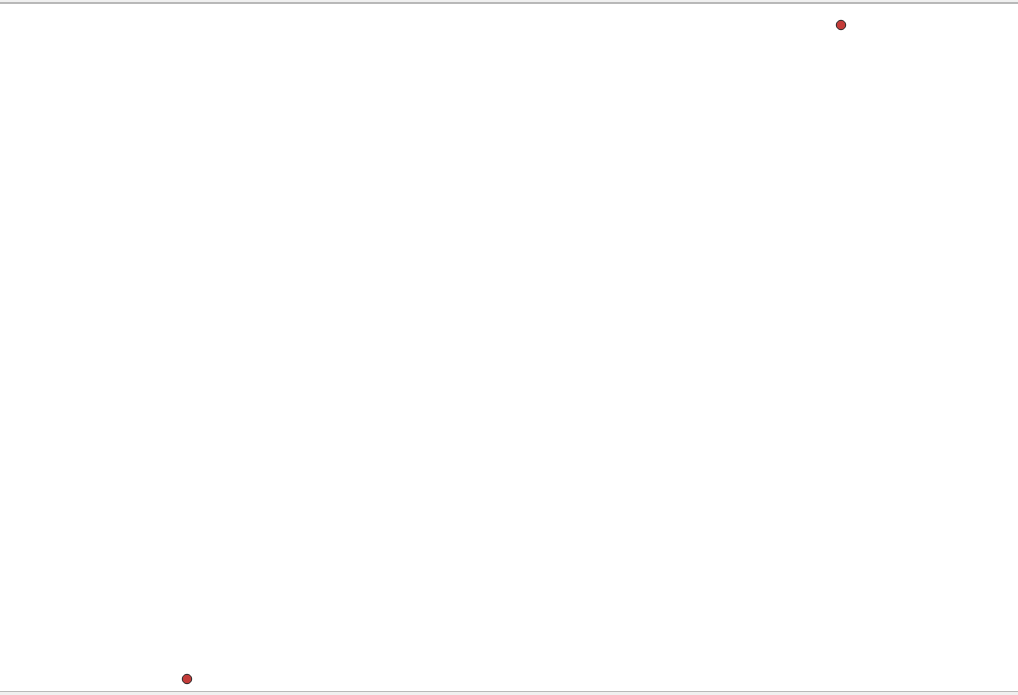
\includegraphics[width=6cm]{figures/Tugas2/1174084/no3.png}
		\centering
		\caption{Point}
	\end{figure}
	\item Nomor 4
	\lstinputlisting{src/tugas2/1174084/soal4.py}
	\begin{figure}[H]
		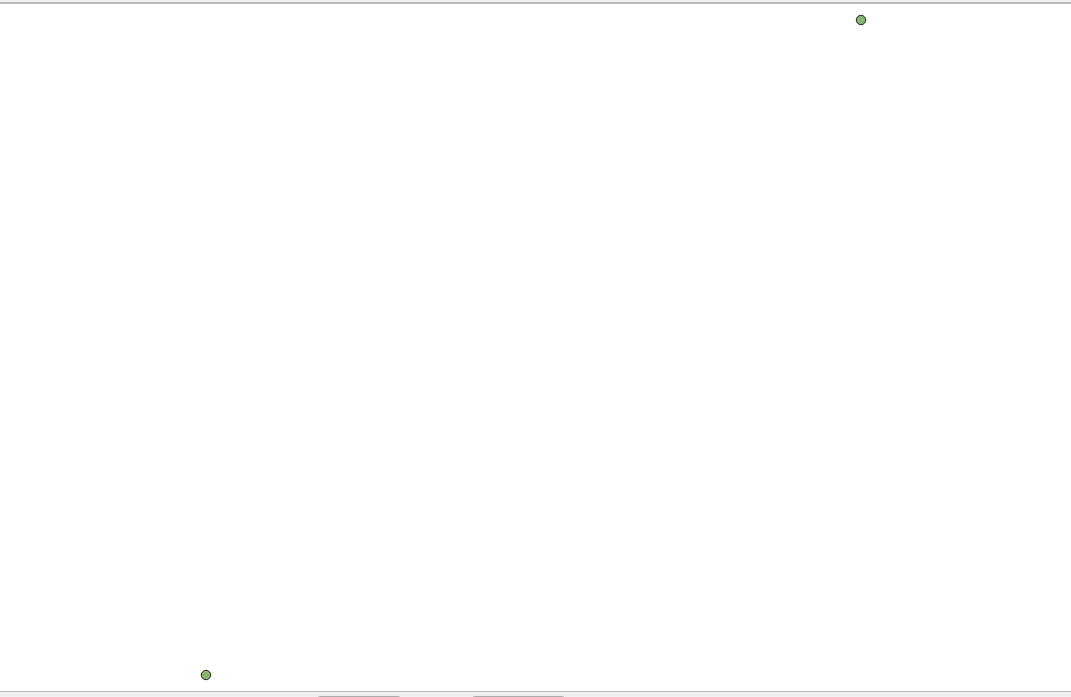
\includegraphics[width=6cm]{figures/Tugas2/1174084/no4.png}
		\centering
		\caption{Point}
	\end{figure}
	\item Nomor 5
	\lstinputlisting{src/tugas2/1174084/soal5.py}
	\begin{figure}[H]
		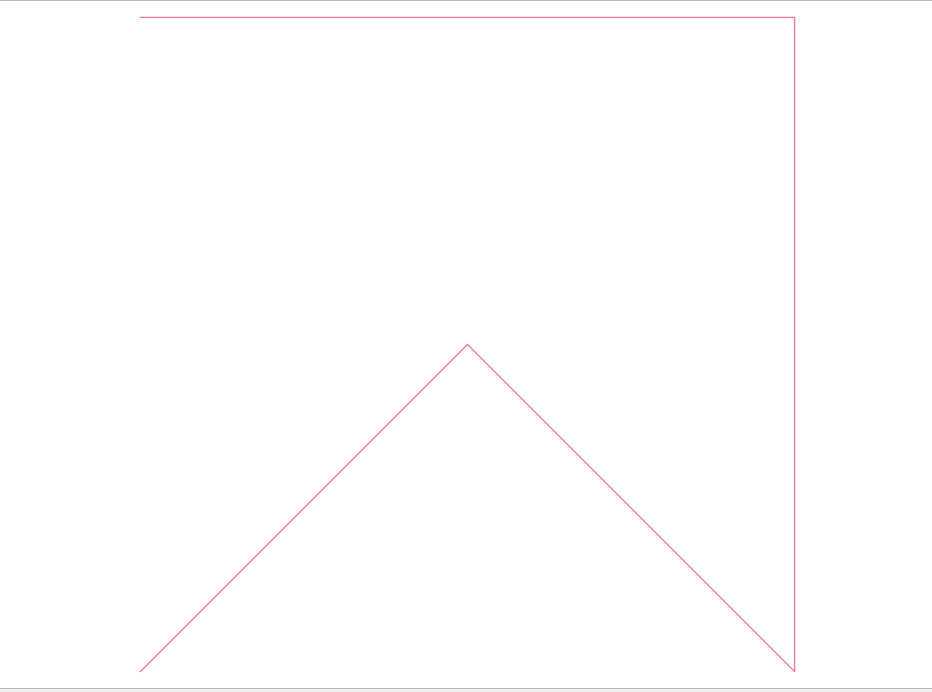
\includegraphics[width=6cm]{figures/Tugas2/1174084/no5.png}
		\centering
		\caption{Polyline}
	\end{figure}
	\item Nomor 6
	\lstinputlisting{src/tugas2/1174084/soal6.py}
	\begin{figure}[H]
		
\includegraphics[width=6cm]{figures/Tugas2/1174084/no6.png}
		\centering
		\caption{Polygon}
	\end{figure}
	\item Nomor 7
	\lstinputlisting{src/tugas2/1174084/soal7.py}
	\begin{figure}[H]
		
\includegraphics[width=6cm]{figures/Tugas2/1174084/no7.png}
		\centering
		\caption{Polygon}
	\end{figure}
	\item Nomor 8
	\lstinputlisting{src/tugas2/1174084/soal8.py}
	\begin{figure}[H]
		
\includegraphics[width=6cm]{figures/Tugas2/1174084/no8.png}
		\centering
		\caption{Polygon}
	\end{figure}
	\item Nomor 9
	\lstinputlisting{src/tugas2/1174084/soal9.py}
	\begin{figure}[H]
		
\includegraphics[width=6cm]{figures/Tugas2/1174084/no9.png}
		\centering
		\caption{Polygon}
	\end{figure}
	\item Nomor 10
	\lstinputlisting{src/tugas2/1174084/soal10.py}
	\begin{figure}[H]
		
\includegraphics[width=6cm]{figures/Tugas2/1174084/no10.png}
		\centering
		\caption{Polygon, Hasil modulus dari npm saya 1174084 adalah 4 jadi membuat bidang jajargenjang dan angka akhir dari npm saya adalah 8 jadi membuat bidangnya sebanyak 8}
	\end{figure}
\end{enumerate}
\subsection{Link}
https://youtu.be/y5qPYgULWOo
